\documentclass[11pt]{article}

\usepackage[a4paper,margin=1in]{geometry}
\usepackage[T1]{fontenc}
\usepackage[utf8]{inputenc}
\usepackage{lmodern}
\usepackage{microtype}
\usepackage{amsmath,amssymb,amsthm,mathtools}
\usepackage{booktabs,tabularx}
\usepackage{adjustbox}
\usepackage{enumitem}
\usepackage{graphicx}
% \usepackage[round,authoryear]{natbib}
\usepackage[numbers]{natbib}
\usepackage{xcolor}
\usepackage{hyperref}

\definecolor{linkblue}{RGB}{20,70,120}
\hypersetup{
  colorlinks=true,
  linkcolor=linkblue,
  citecolor=linkblue,
  urlcolor=linkblue,
  pdftitle={Two-Space Faithfulness in Projector-Based Self-Supervised Learning},
  pdfauthor={Anonymous Authors}
}
\urlstyle{same}

\setlength{\parindent}{1.2em}
\setlength{\parskip}{0pt}
\setlist[itemize]{leftmargin=*,topsep=3pt,itemsep=2pt}
\setlist[enumerate]{leftmargin=*,topsep=3pt,itemsep=2pt}
\numberwithin{equation}{section}

\newtheorem{theorem}{Theorem}[section]
\newtheorem{proposition}[theorem]{Proposition}

\newenvironment{takeaway}
{\par\smallskip\noindent\begin{minipage}{\linewidth}\hrule\smallskip\textbf{Takeaway.}\ }
{\smallskip\hrule\end{minipage}\par\smallskip}

\newcommand{\TODO}[1]{\textcolor{red!70!black}{\textbf{TODO:} #1}}
\newcommand{\R}{\mathbb{R}}
\newcommand{\E}{\mathbb{E}}
\newcommand{\Cov}{\operatorname{Cov}}
\newcommand{\tr}{\operatorname{tr}}
\newcommand{\srank}{\operatorname{srank}}
\newcommand{\range}{\operatorname{range}}
\newcommand{\cM}{\mathcal{M}}
\newcommand{\cL}{\mathcal{L}}
\newcommand{\cK}{\mathcal{K}}
\newcommand{\cE}{\mathcal{E}}
\newcommand{\norm}[1]{\lVert #1\rVert}
\newcommand{\argmin}{\operatorname*{arg\,min}}


\title{Two-Space Faithfulness in Projector-Based Self-Supervised Learning}
\author{Author Name}
\date{}

\begin{document}
\maketitle

\begin{abstract}
Projector-based self-supervised learning (SSL) optimizes a projected representation
$Z=p(H)$ but typically discards the projector and retains the backbone $H$.
Properties enforced in $Z$ therefore need not hold in the representation used
downstream. We formalize this gap through factorization non-identifiability and
measure the missing cross-space relation by held-out linear accessibility.

We then introduce representation-level moment regularization applied directly to
the stable source-center geometry of both $H$ and $Z$. If
$C_s=B_s+A_s$ separates across-source center variation $B_s$ from within-source
augmentation variation $A_s$, pooling $V$ independent views yields covariance
$B_s+A_s/V$, allowing moment control to target stable capacity rather than
marginal spread alone. Finally, we characterize the retained backbone by its
normalized augmentation thickness
$\Theta_h=B_h^{\dagger/2}A_hB_h^{\dagger/2}$. A compact two-sided result shows
that too little thickness can exclude distinctions that are difficult under the
augmentation channel, while too much thickness increases linear readout error
once center organization is fixed. Empirically, direct representation
regularization preserves capacity and improves existing SSL methods, moves
retained augmentation geometry in a favorable direction, and can also be used
in the projected space as part of a competitive standalone SSL objective.
\end{abstract}

\section{Introduction}\label{sec:intro}

Projector-based SSL typically computes
\[
H=h(V),\qquad Z=p(H),
\]
applies the pretraining objective to $Z$, and retains $H$ downstream
\citep{simclr2020,vicreg2022,xue2024,ouyang2025}. This creates a simple mismatch:
the representation directly constrained during training is not the
representation ultimately evaluated.

Our starting point is that a $Z$-only objective cannot in general certify a
non-invariant property of $H$. Distinct backbone--projector factorizations can
produce the same projected variables while changing covariance, rank,
Gaussianity, margins, or linearly available information in the backbone. Rather
than assuming that projected-space structure transfers, we measure whether it is
linearly accessible from $H$ after training.

This motivates direct control of the representation that is actually retained.
For $S\in\{H,Z\}$, we separate stable source-center spread from augmentation
variation,
\[
B_s=\Cov(\E[S\mid Q]),\qquad
A_s=\E[\Cov(S\mid Q)],\qquad
C_s=B_s+A_s.
\]
Marginal spread $C_s$ can remain large even if stable source distinctions in
$B_s$ collapse. We therefore regularize pooled representation centers directly.
For $V$ independent views of the same source, their pooled covariance is
$B_s+A_s/V$, so increasing the number of pooled views suppresses augmentation
noise and exposes the stable geometry.

The same decomposition also gives a scale for retained augmentation sensitivity:
\[
\Theta_h=B_h^{\dagger/2}A_hB_h^{\dagger/2}.
\]
Unlike raw augmentation variance, $\Theta_h$ measures within-source variation
relative to stable image-to-image separation. We use it as the main geometric
quantity for explaining the retained representation: useful features need not
be maximally invariant, but neither should augmentation variation dominate
their stable organization.

\paragraph{Contributions.}
We make four claims.
\begin{itemize}
\item We formalize why projected-space guarantees do not, by themselves,
identify the retained backbone, and use held-out linear accessibility to measure
when projected organization is available from $H$.
\item We introduce moment regularization applied directly to learned
representations, including the retained backbone, and show why pooled-center
regularization protects stable source-center capacity in both $H$ and $Z$.
\item We use normalized augmentation thickness $\Theta_h$ to give a lean
two-sided account of retained representation strength: too little thickness
rules out sufficiently augmentation-difficult distinctions, while too much
thickness hurts linear readout for fixed center organization.
\item Empirically, the same intervention improves capacity and downstream
performance across existing SSL methods; applying the representation-level
regularizer in $Z$ as well yields our standalone SSL objective.
\end{itemize}

\section{The projector gap and cross-space accessibility}\label{sec:gap}

A $Z$-only objective sees the backbone--projector pair only through $p\circ h$.
The backbone geometry is therefore not identified by the projected variables
alone.

\begin{theorem}[$Z$-only objectives identify only the projected factorization class]
\label{thm:discrepancy}
Suppose an objective $J(h,p)$ depends on $(h,p)$ only through
$Z=p(h(V))$. If another admissible pair $(\widetilde h,\widetilde p)$ satisfies
\[
\widetilde p(\widetilde h(V))=p(h(V))
\]
pathwise, then
\[
J(\widetilde h,\widetilde p)=J(h,p).
\]
Hence a backbone property can be uniformly certified by a $Z$-only objective
only if it is constant over every admissible factorization of the same projected
map.
\end{theorem}

The obstruction already appears under invertible reparameterizations, mappings
that discard backbone information, and extra backbone coordinates ignored by
the projector. Explicit fixed-$Z$ examples for Gaussianity and linear
separability are deferred to Appendix~\ref{app:discrepancy}. The point is not
that projector-based SSL fails, but that a separate cross-space statement is
needed before transferring a property from $Z$ to $H$.

We measure that statement at the level of source centers. Assume $B_z$ has rank
$r_z$ and whiten projected centers so that
$\Cov(\overline m_z(Q))=I_{r_z}$. Let
\[
W_c
=
\argmin_W
\E\norm{\overline m_z(Q)-W(m_h(Q)-\mu_h)}^2,
\]
with residual covariance
\[
\Sigma_c
=
\Cov\!\left(
\overline m_z(Q)-W_c(m_h(Q)-\mu_h)
\right).
\]
We summarize average accessibility by
\begin{equation}\label{eq:average-access}
R^2_{\rm acc}
=
1-\frac{\tr\Sigma_c}{r_z}.
\end{equation}
For a particular projected direction $u$, the unexplained variance is exactly
$u^\top\Sigma_cu$.

To state the corresponding transfer result, let $\cM_z$ and $\cM_h$ denote the
linear spans of the projected and backbone source-center coordinates, and define
\[
d_s(y)=\min_{g\in\cM_s}\norm{y-g}_{L^2},
\qquad s\in\{h,z\},
\]
for a centered source target $y$. If
$P_{\cM_z}y=u_y^\top\overline m_z(Q)$, least squares gives
\begin{equation}\label{eq:organization-transfer}
d_h(y)
\le
d_z(y)+\sqrt{u_y^\top\Sigma_cu_y}.
\end{equation}
Thus projected organization transfers to the retained backbone whenever the
relevant projected direction is linearly accessible. In experiments we estimate
this relation on held-out source centers.

\begin{takeaway}
A property established in $Z$ is not automatically a property of $H$.
Accessibility provides the missing empirical bridge without treating it as a
definition of representation quality.
\end{takeaway}

\section{Direct representation regularization in both spaces}
\label{sec:regularization}

Let $Q$ index source images and $V\sim\mathsf A(\cdot\mid Q)$ an augmented view.
For $S\in\{H,Z\}$ define
\[
m_s(Q)=\E[S\mid Q],\qquad
B_s=\Cov(m_s(Q)),\qquad
A_s=\E[\Cov(S\mid Q)].
\]
Then
\begin{equation}\label{eq:cov-decomp}
C_s:=\Cov(S)=B_s+A_s.
\end{equation}
The distinction matters because $C_s$ can be nondegenerate purely through
within-source variation even when stable source-center structure in $B_s$ is
poor.

For $V$ conditionally independent views of the same source, let
\[
\overline S_V=\frac1V\sum_{v=1}^V S^{(v)}.
\]
Then
\begin{equation}\label{eq:pooled-cov-main}
\Cov(\overline S_V)=B_s+\frac1V A_s.
\end{equation}
Thus moment control on pooled representation centers increasingly targets stable
source-center geometry as $V$ grows.

We use the log-determinant moment penalty
\begin{equation}\label{eq:moment-penalty}
\cK_{\rm ctr}(\mu,\widetilde B)
=
\frac12\left(
\norm{\mu}^2+\tr\widetilde B-\log\det\widetilde B-d
\right),
\end{equation}
where $\widetilde B$ is the pooled-center covariance on the active
$d$-dimensional subspace. The log-determinant term acts as a spectral barrier
against vanishing directions. Crucially, this penalty is applied to
\emph{representation statistics themselves}; in particular, we apply it
directly to the retained backbone $H$, rather than only to the projector output
or to encoder weights.

The finite-view effect is transparent in the whitening limit.

\begin{proposition}[Pooled-center control protects stable capacity]
\label{prop:capacity-main}
If
\[
\mu_s=0,\qquad
\Cov(\overline S_V)=I_d,\qquad
\norm{A_s}_{\rm op}\le\alpha<V,
\]
then
\[
\left(1-\frac{\alpha}{V}\right)I_d
\preceq B_s\preceq I_d,
\qquad
\srank(B_s)\ge d\left(1-\frac{\alpha}{V}\right).
\]
\end{proposition}

The finite-loss extension is deferred to Appendix~\ref{app:capacity}. Applied
in both $H$ and $Z$, this gives the capacity needed for a nondegenerate
cross-space comparison.

Our training objective is
\begin{equation}\label{eq:objective}
\cL
=
\cL_{\rm pair}(Z_1,\ldots,Z_V)
+
\lambda_z\cK_{\rm ctr}(
\widehat\mu_z,\widehat B_{z,V_z}^{\rm train})
+
\lambda_h\cK_{\rm ctr}(
\widehat\mu_h,\widehat B_{h,V_h}^{\rm train}).
\end{equation}
We use this in two ways. For existing SSL methods, the backbone term can be
added while leaving the method's projected objective unchanged. The same
representation-level moment control can also be used in $Z$, together with the
pairwise agreement term, to form our standalone SSL objective. Estimation and
implementation details are deferred to Appendix~\ref{app:experiments}.

\section{Normalized augmentation thickness}
\label{sec:thickness}

The regularizer was introduced to preserve stable capacity, but it also changes
how augmentation variation is retained in $H$. Raw within-source variance is
not meaningful on its own: the same augmentation spread has a different effect
when source centers are far apart than when they are tightly packed. We
therefore normalize by stable center geometry:
\begin{equation}\label{eq:theta}
\Theta_h
=
B_h^{\dagger/2}A_hB_h^{\dagger/2}.
\end{equation}
Equivalently, along any stable direction $a$,
\[
\lambda_h(a)
=
\frac{a^\top A_ha}{a^\top B_ha}
\]
is augmentation variation measured relative to source-center variation.

For the compact theory below, whiten the active center subspace so that
\[
\overline H=\overline m_h(Q)+\xi_h,\qquad
\Cov(\overline m_h)=I,\qquad
\Cov(\xi_h)=\Theta_h.
\]
For a centered source target $y$, define its augmentation difficulty
\begin{equation}\label{eq:view-difficulty}
\cE_{\mathsf A}(y)
=
\min_{f}
\E[(y(Q)-f(V))^2],
\end{equation}
the irreducible error of recovering that source distinction from a single
augmented view. Let
\[
d_h(y)=\min_{g\in\cM_h}\norm{y-g}_{L^2}
\]
measure whether the distinction is organized by the backbone source centers.

The following two statements are the only properties of $\Theta_h$ that we need
in the main text.

\begin{theorem}[Two sides of retained augmentation thickness, per direction]
\label{thm:retained-resolution}
Let $y$ be centered with $\norm{y}_{L^2}\le1$, let $P_{\cM_h}y=a^\top\overline m_h(Q)$ be
its projection onto the backbone center span, and let
\[
\lambda_h(a)=\frac{a^\top\Theta_ha}{\norm{a}^2}
\]
be the retained thickness along the direction that reads $y$ from the centers (in the
original coordinates this is $u^\top A_hu/u^\top B_hu$ for the center reader $u$). Then
$\norm{a}^2=\norm{y}^2-d_h(y)^2$, and:
\begin{enumerate}[label=(\roman*)]
\item \textbf{One identity.} The best linear single-view read of $y$ costs
\begin{equation}\label{eq:organization-thickness-decomp}
\inf_u
\E[(y-u^\top\overline H)^2]
=
d_h(y)^2
+
a^\top\Theta_h(I+\Theta_h)^{-1}a,
\qquad
a^\top\Theta_h(I+\Theta_h)^{-1}a\le\norm{a}^2\lambda_h(a):
\end{equation}
center error plus thickness along the reader, and nothing else.

\item \textbf{Too thin.} No single-view predictor beats the augmentation difficulty, so
\begin{equation}\label{eq:too-thin-main}
d_h(y)^2
\;\ge\;
\cE_{\mathsf A}(y)-a^\top\Theta_h(I+\Theta_h)^{-1}a
\;\ge\;
\cE_{\mathsf A}(y)-\norm{a}^2\lambda_h(a)
\;\ge\;
\cE_{\mathsf A}(y)-\lambda_h(a).
\end{equation}
Equivalently, a representation organizes $y$ to center error $d_h(y)$ only if its
thickness along the reader covers the difficulty that organization has not paid,
\[
\lambda_h(a)\;\ge\;\frac{\cE_{\mathsf A}(y)-d_h(y)^2}{\norm{y}^2-d_h(y)^2}.
\]
The worst-direction form $d_h(y)\ge(\sqrt{\cE_{\mathsf A}(y)}-\sqrt{\norm{\Theta_h}_{\rm op}})_+$
follows, since $\lambda_h(a)\le\norm{\Theta_h}_{\rm op}$ and
$\cE-\lambda\ge(\sqrt{\cE}-\sqrt{\lambda})_+^2$; it is never tighter.

\item \textbf{Too thick.} For fixed center organization and reading direction $a$, the
second term of \eqref{eq:organization-thickness-decomp} is monotone nondecreasing in
$\Theta_h$ under the PSD order.
\end{enumerate}
\end{theorem}

Both sides are one identity read in two directions. A single-view read of a distinction
costs its center error plus the thickness along the direction that reads it. That sum can
never fall below the augmentation difficulty of the distinction, so thickness along the
reader is necessary for whatever the augmentation blurs and the centers organize (too
thin); and for fixed organization the same term is what a single view pays (too thick).
Thickness enters only along reading directions. Directions in which views spread far more
than images, the tail of the thickness spectrum, do not enter unless a task reads them,
which is why the worst-direction form says nothing on trained models while the
per-direction form does. The first inequality in \eqref{eq:too-thin-main} is an equality
exactly when the best linear single-view read of the representation is the Bayes
predictor of $y$ from a view. Proofs and estimator details are deferred to
Appendix~\ref{app:resolution}.

\begin{takeaway}
$\Theta_h$ is the scale on which augmentation sensitivity should be judged:
neither maximal invariance nor unconstrained within-source spread is the right
target.
\end{takeaway}

\section{Experiments}\label{sec:experiments}

% Skeleton opened 2026-08-24 (text: Berker). Figures/tables auto-generated by
% experiments/paper_exhibits.py from the standing result CSVs.

\subsection{Setup}\label{sec:exp-setup}
% STORY BEAT: one yardstick, matched frames. Frames (IN-100 zoo ViT-S/16 100ep matched;
% IN-1k S/B/L); the single evaluation protocol for every IN-1k row (bench_linear_v1 +
% kNN-200 t=.07); the epoch-matched external block (OK-AI unified-codebase revisions);
% transfer/OOD/seg follow the VISReg protocols, cited rows marked, self-run matched-impl
% elsewhere; the battery metrics used later (Theta, EffRank, d_h) each get one plain
% sentence here so no later section defines notation mid-claim.

\subsection{The discrepancy: the stated desideratum lives in $Z$}\label{sec:exp-discrepancy}
\begin{figure}[t]
  \centering
  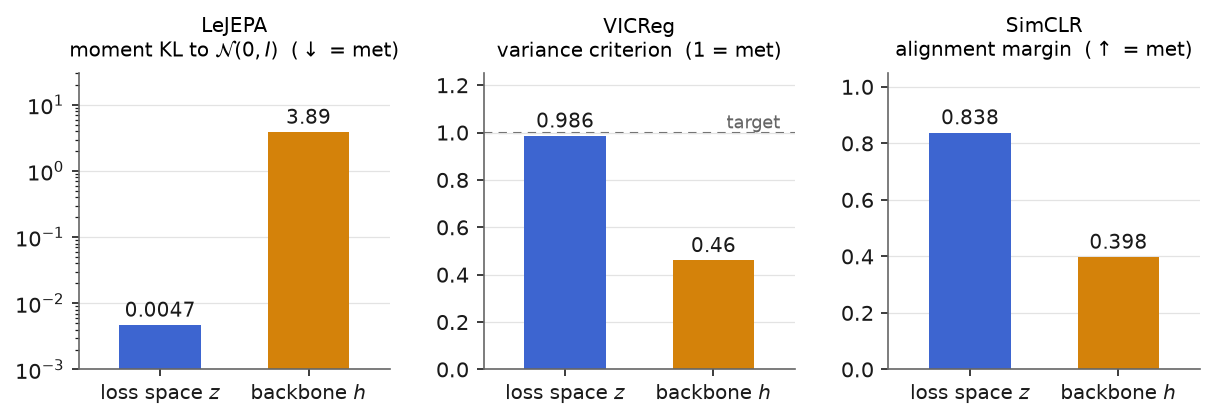
\includegraphics[width=0.9\linewidth]{figures/fig_discrepancy.png}
  \caption{}\label{fig:discrepancy}
\end{figure}

\subsection{Treatment: before and after on existing methods}\label{sec:exp-treatment}
% STORY BEAT: the h-side moment floor, added to five view-based methods + ours pair,
% protects stable center capacity (x1.8-5.4 kept-rank, all pairs) and improves probes
% (kNN: five risers one flat; linear: four risers, DINO* = the recorded overshoot dose,
% redo in flight). Accessibility improves where headroom exists, never hurts. Figures:
% fig:treatment (metric grid), fig:treatment-arrows (the movement view).
\begin{figure}[t]
  \centering
  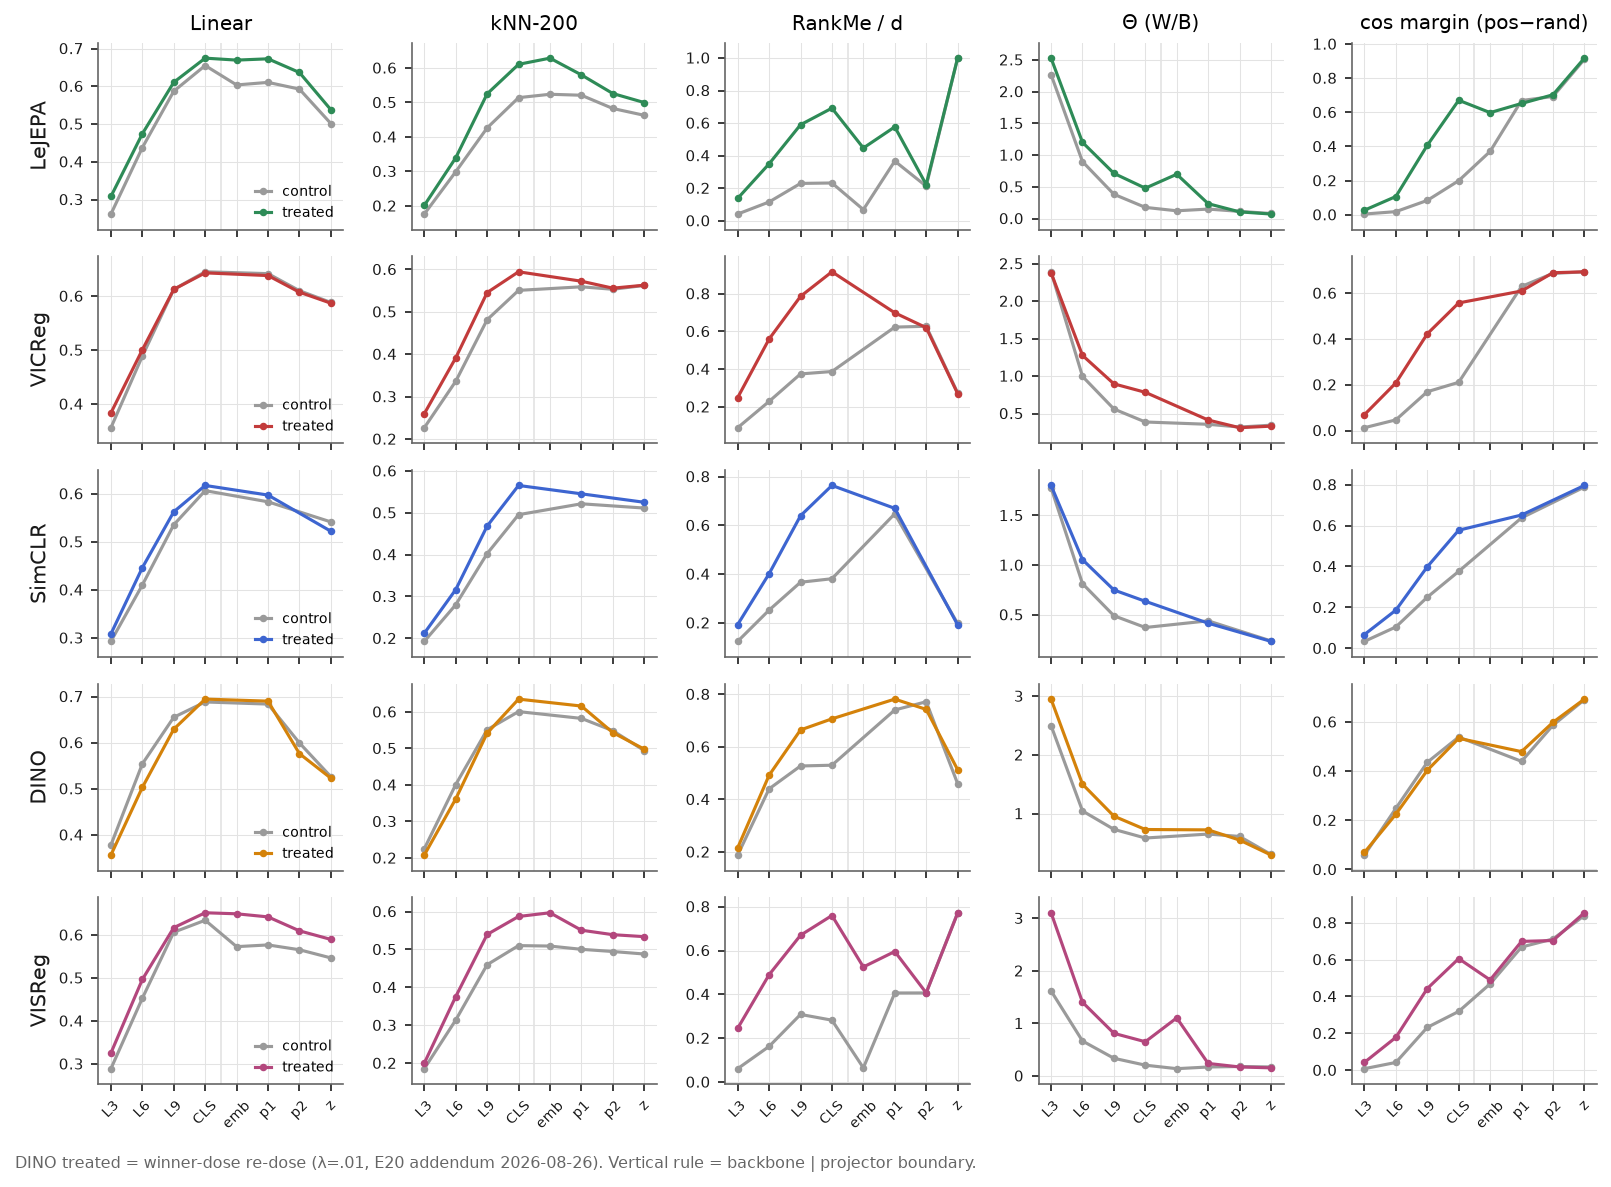
\includegraphics[width=\linewidth]{figures/fig_treatment_main.png}
  \caption{}\label{fig:treatment}
\end{figure}
% exhaustive per-metric version: Fig.~\ref{fig:treatment-appendix} (appendix).

\begin{figure}[t]
  \centering
  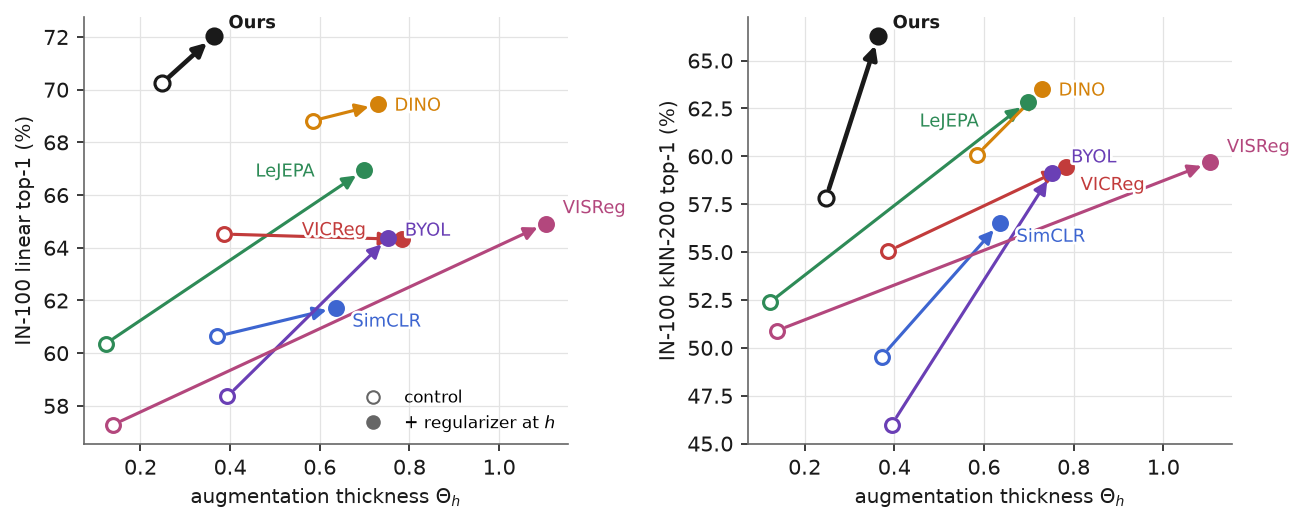
\includegraphics[width=\linewidth]{figures/fig_treatment_arrows.png}
  \caption{The moment floor moves every view-based method through
  $(\Theta_h,\ \text{accuracy})$ space (IN-100, matched frame and epochs; open =
  control, filled = treated): linear top-1 (left) and kNN-200 (right).
  $^*$DINO's treated arm ran the recorded overshoot dose.}\label{fig:treatment-arrows}
\end{figure}

\subsection{Where the improvement comes from}\label{sec:exp-mechanism}
% STORY BEAT: per class, single-view probe error splits EXACTLY (identity, corr .99)
% into center organization + view-sensitivity along that class's own direction. The
% treatment improves organization (-.08..-.17) at a small sensitivity shift (+.01..+.06)
% in all six pairs; 96/100 classes improve for our pair. This kills the thickness-
% monotonicity reading in both directions and is the task-anchored mechanism claim.
% C8 term-shift panel to be added beside fig:org-sensitivity when rebuilt.
\begin{figure}[t]
  \centering
  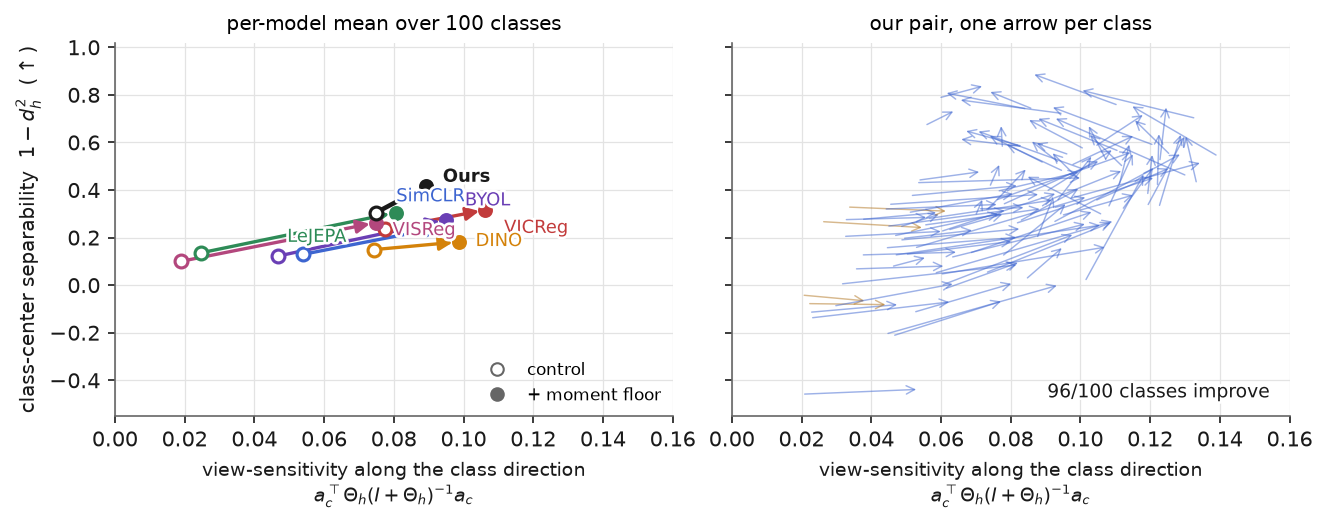
\includegraphics[width=\linewidth]{figures/fig_org_vs_sensitivity.png}
  \caption{Class-center separability against view-sensitivity along each class's own
  readout direction. Left: per-model means over 100 classes (control $\to$ treated).
  Right: our pair, one arrow per class. No monotone relation between the two quantities
  is claimed; organization gains dominate the accompanying sensitivity
  shift.}\label{fig:org-sensitivity}
\end{figure}

\subsection{ImageNet-1k at scale}\label{sec:exp-in1k}
% STORY BEAT: everything on our single yardstick (tab:in1k-main): the epoch-matched
% 100-ep block (OK-AI + the certified Lightly repro + ours), the 300/400-ep field, and
% the 400-ep runs landing 09-06..13 filling the Ours rows; epoch scaling contextualized
% by VISReg's measured +4.3 (100->400) on the same yardstick. tab:placement = the
% structure metrics for every public row (the external read of the theory's axes).
\begin{table}[t]
  \centering
  \small
% BEGIN placement-table (auto-generated by experiments/paper_exhibits.py — edit there)
\begin{adjustbox}{max width=\textwidth}
\begin{tabular}{lrrrrrrrrrrr}
\toprule
Method & Ep. & Linear & kNN-200 & RankMe/d & EffRank/d & Gauss. KL & Epps–Pulley & Kurt. (worst) & cos margin & class margin & $\Theta$ \\
\midrule
Ours (ViT-S/16) & 100 & 0.663 & 0.545 & 0.903 & 0.739 & 0.229 & 44.6 & 3.564 & 0.813 & 0.375 & 0.211 \\
Ours (ViT-S/16, 10 views) & 100 & 0.685 & 0.577 & 0.933 & 0.806 & 0.153 & 895.0 & 7.727 & 0.832 & 0.404 & 0.185 \\
LeJEPA (Lightly benchmark repro.) & 100 & 0.641 & 0.471 & 0.586 & 0.324 & 3.192 & 3607.8 & 1.013 & 0.176 & 0.082 & 0.318 \\
LeJEPA (OK-AI, ViT-S/16) & 300 & 0.664 & 0.515 & 0.783 & 0.315 & 0.841 & 2635.8 & 0.885 & 0.770 & 0.431 & 0.230 \\
DINO (OK-AI, ViT-S/16) & 300 & 0.738 & 0.710 & 0.951 & 0.857 & 2.668 & 291.6 & 0.171 & 0.637 & 0.229 & 0.555 \\
iBOT (OK-AI, ViT-S/16) & 300 & 0.752 & 0.715 & 0.868 & 0.704 & 2.646 & 530.0 & 0.242 & 0.681 & 0.282 & 0.452 \\
MoCo v3 (ViT-S/16) & 300 & 0.732 & 0.648 & 0.596 & 0.524 & 2.935 & 872.2 & 0.782 & 0.091 & 0.045 & 0.277 \\
LeJEPA (OK-AI, ViT-B/16) & 300 & 0.724 & 0.594 & 0.758 & 0.261 & 1.087 & 2360.1 & 0.943 & 0.773 & 0.426 & 0.216 \\
MoCo v3 (ViT-B/16) & 300 & 0.759 & 0.682 & 0.727 & 0.507 & 3.079 & 825.5 & 0.844 & 0.265 & 0.113 & 0.319 \\
DINO (ViT-B/16) & 400 & 0.772 & 0.733 & 0.786 & 0.463 & 2.009 & 725.9 & 2.616 & 0.671 & 0.374 & 0.390 \\
iBOT (ViT-B/16) & 400 & 0.785 & 0.748 & 0.830 & 0.490 & 2.079 & 475.2 & 0.986 & 0.707 & 0.397 & 0.342 \\
VISReg (ViT-B/16) & 400 & 0.746 & 0.600 & 0.693 & 0.238 & 0.886 & 2182.7 & 0.882 & 0.511 & 0.280 & 0.129 \\
iBOT (ViT-L/16) & 250 & 0.795 & 0.749 & 0.802 & 0.442 & 2.050 & 581.3 & 0.886 & 0.700 & 0.423 & 0.309 \\
VISReg (ViT-L/16) & 400 & 0.754 & 0.604 & 0.613 & 0.191 & 1.358 & 2018.4 & 3.588 & 0.311 & 0.161 & 0.101 \\
\bottomrule
\end{tabular}
\end{adjustbox}
% END placement-table
  \caption{}\label{tab:placement}
\end{table}

\subsection{Transfer, robustness, and dense prediction}\label{sec:exp-transfer}
% STORY BEAT: the same checkpoints under the VISReg downstream protocols — the eight
% transfer sets (tab:transfer), the six domain-shift sets (tab:ood), ADE20k segmentation
% (tab:seg); cited baselines marked, ours self-run under the matched implementation with
% a reproduced validation cell per protocol.
\begin{table}[t]
  \centering
  \small
% BEGIN transfer-table (auto-generated by experiments/paper_exhibits.py — edit there;
% VISReg Table-5 downstream suite under their 10-ep concat-4-CLS LP protocol; baseline
% cells cited where published (marked), self-run under the matched implementation else)
\begin{adjustbox}{max width=\textwidth}
\begin{tabular}{llrrrrrrrrrr}
\toprule
Method & Backbone & Ep. & DTD & Aircraft & Cars & CIFAR10 & CIFAR100 & Flowers & Food & Pets & Avg. \\
\midrule
MoCo v3$^\ddag$ & ViT-B/16 & 300 & 73.7 & 57.9 & 67.5 & 96.9 & 85.2 & 91.5 & 81.8 & 89.8 & 80.5 \\
DINO$^\ddag$ & ViT-B/16 & 400 & 74.3 & 63.6 & 73.9 & 96.5 & 85.0 & 94.6 & 83.1 & 93.6 & 83.1 \\
iBOT$^\ddag$ & ViT-B/16 & 400 & 74.1 & 63.5 & 73.8 & 97.1 & 85.9 & 93.7 & 84.2 & 93.6 & 83.2 \\
iBOT$^\ddag$ & ViT-L/16 & 250 & 75.3 & 66.0 & 76.1 & 97.5 & 87.2 & 94.0 & 86.1 & 94.0 & 84.5 \\
I-JEPA$^\ddag$ & ViT-H/14 & 300 & 69.9 & 55.4 & 59.2 & 97.2 & 85.5 & 86.8 & 83.3 & 92.8 & 78.7 \\
data2vec$^\ddag$ & ViT-L/14 & 1600 & 69.7 & 43.9 & 38.7 & 96.9 & 83.7 & 81.4 & 79.6 & 83.0 & 72.1 \\
MAE$^\ddag$ & ViT-L/16 & 1600 & 72.8 & 61.9 & 61.5 & 93.3 & 78.0 & 85.4 & 78.6 & 91.3 & 77.8 \\
VISReg$^\ddag$ & ViT-B/16 & 400 & 75.7 & 57.1 & 64.8 & 94.6 & 78.8 & 90.4 & 82.9 & 88.3 & 79.1 \\
VISReg$^\ddag$ & ViT-L/14 & 400 & 76.5 & 56.6 & 66.2 & 94.1 & 71.9 & 90.2 & 83.3 & 89.2 & 78.5 \\
LeJEPA$^\ddag$ & ViT-L/14 & 100 & 78.3 & 57.0 & 57.3 & 96.5 & 83.7 & 91.2 & 82.1 & 89.7 & 79.5 \\
\midrule
VISReg (repro.) & ViT-B/16 & 100 & 73.3 & 53.1 & 58.0 & 94.3 & 79.6 & 87.9 & 79.1 & 85.5 & 76.4 \\
Ours & ViT-S/16 & 100 & 71.1 & 55.5 & 62.5 & 95.3 & 81.6 & 90.4 & 75.3 & 89.1 & 77.6 \\
Ours & ViT-S/16 & 400 & --- & --- & --- & --- & --- & --- & --- & --- & --- \\
Ours & ViT-B/16 & 100 & 71.5 & 59.8 & 71.1 & 96.7 & 84.9 & 92.2 & 79.4 & 91.7 & 80.9 \\
Ours & ViT-B/16 & 400 & 73.2 & 61.1 & 74.0 & 96.9 & 85.4 & 92.0 & 81.0 & 92.2 & 82.0 \\
Ours & ViT-L/16 & 100 & --- & --- & --- & --- & --- & --- & --- & --- & --- \\
Ours & ViT-L/16 & 400 & --- & --- & --- & --- & --- & --- & --- & --- & --- \\
\bottomrule
\end{tabular}
\end{adjustbox}
% END transfer-table
  \caption{Transfer linear probing on the eight downstream classification sets
  (top-1; Avg.\ over the eight), under the VISReg evaluation protocol (concatenated
  CLS of the last 4 blocks, 10-epoch linear probe, LR grid). $^\ddag$Numbers as
  reported by the VISReg paper; unmarked rows are evaluated by us under the matched
  implementation.}\label{tab:transfer}
\end{table}


\begin{table}[t]
  \centering
  \small
% BEGIN in1k-main-table (auto-generated by experiments/paper_exhibits.py — edit there;
% external rows = public checkpoints under our bench_linear_v1 yardstick; Ours 400-ep
% cells fill as the D-103 runs land ~09-05..12)
\begin{tabular}{llrrr}
\toprule
Method & Backbone & Ep. & Linear & kNN \\
\midrule
LeJEPA (OK-AI) & ViT-S/16 & 100 & 62.5 & 45.5 \\
DINO (OK-AI) & ViT-S/16 & 100 & 70.0 & 64.7 \\
iBOT (OK-AI) & ViT-S/16 & 100 & 70.9 & 65.7 \\
LeJEPA (Lightly repro.) & ViT-S/16 & 100 & 64.1 & 47.1 \\
Ours & ViT-S/16 & 100 & 69.7 & 59.2 \\
Ours & ViT-S/16 & 400 & --- & --- \\
\midrule
LeJEPA (OK-AI) & ViT-B/16 & 100 & 69.7 & 51.3 \\
DINO (OK-AI) & ViT-B/16 & 100 & 73.9 & 69.4 \\
iBOT (OK-AI) & ViT-B/16 & 100 & 77.0 & 72.9 \\
LeJEPA (OK-AI) & ViT-B/16 & 300 & 72.4 & 59.4 \\
MoCo v3 & ViT-B/16 & 300 & 75.9 & 68.2 \\
DINO & ViT-B/16 & 400 & 77.2 & 73.3 \\
iBOT & ViT-B/16 & 400 & 78.5 & 74.8 \\
VISReg & ViT-B/16 & 400 & 74.6 & 60.0 \\
VISReg (repro.) & ViT-B/16 & 100 & 70.3 & 52.5 \\
Ours & ViT-B/16 & 100 & 74.2 & 64.3 \\
Ours & ViT-B/16 & 400 & 76.0 & 68.6 \\
\midrule
iBOT & ViT-L/16 & 250 & 79.5 & 74.9 \\
VISReg & ViT-L/14 & 400 & 75.4 & 60.4 \\
MAE & ViT-L/16 & 1600 & 75.7 & 46.4 \\
LeJEPA$^\dagger$ & ViT-L/14 & 100 & 75.6 & --- \\
I-JEPA$^\dagger$ & ViT-H/14 & 300 & 79.3 & --- \\
\midrule
Ours & ViT-L/16 & 100 & --- & --- \\
Ours & ViT-L/16 & 400 & --- & --- \\
\bottomrule
\end{tabular}
% END in1k-main-table
  \caption{ImageNet-1k linear and kNN (k=200, t=.07) top-1 under a single evaluation
  protocol (bench\_linear\_v1) for all rows. $^\dagger$Published numbers from the
  respective papers; not evaluated under our protocol.}\label{tab:in1k-main}
\end{table}

\begin{table}[t]
  \centering
  \small
% BEGIN ood-table (auto-generated by experiments/paper_exhibits.py — edit there;
% skeleton: the bench-trained linear head evaluated on the ImageNet shift suite)
\begin{tabular}{llrrrrrrr}
\toprule
Method & Backbone & Ep. & ChestX & RetinaMNIST & OrganAMNIST & Galaxy10 & AID & DTD \\
\midrule
LeJEPA (OK-AI) & ViT-S/16 & 100 & --- & --- & --- & --- & --- & --- \\
DINO (OK-AI) & ViT-S/16 & 100 & --- & --- & --- & --- & --- & --- \\
iBOT (OK-AI) & ViT-S/16 & 100 & --- & --- & --- & --- & --- & --- \\
LeJEPA (Lightly repro.) & ViT-S/16 & 100 & --- & --- & --- & --- & --- & --- \\
Ours & ViT-S/16 & 100 & --- & --- & --- & --- & --- & --- \\
Ours & ViT-S/16 & 400 & --- & --- & --- & --- & --- & --- \\
\midrule
LeJEPA (OK-AI) & ViT-B/16 & 100 & --- & --- & --- & --- & --- & --- \\
DINO (OK-AI) & ViT-B/16 & 100 & --- & --- & --- & --- & --- & --- \\
iBOT (OK-AI) & ViT-B/16 & 100 & --- & --- & --- & --- & --- & --- \\
LeJEPA (OK-AI) & ViT-B/16 & 300 & --- & --- & --- & --- & --- & --- \\
MoCo v3 & ViT-B/16 & 300 & --- & --- & --- & --- & --- & --- \\
DINO & ViT-B/16 & 400 & --- & --- & --- & --- & --- & --- \\
iBOT & ViT-B/16 & 400 & --- & --- & --- & --- & --- & --- \\
VISReg & ViT-B/16 & 400 & --- & --- & --- & --- & --- & --- \\
VISReg (repro.) & ViT-B/16 & 100 & --- & --- & --- & --- & --- & --- \\
Ours & ViT-B/16 & 100 & --- & --- & --- & --- & --- & --- \\
Ours & ViT-B/16 & 400 & --- & --- & --- & --- & --- & --- \\
\midrule
iBOT & ViT-L/16 & 250 & --- & --- & --- & --- & --- & --- \\
VISReg & ViT-L/14 & 400 & --- & --- & --- & --- & --- & --- \\
MAE & ViT-L/16 & 1600 & --- & --- & --- & --- & --- & --- \\
LeJEPA$^\dagger$ & ViT-L/14 & 100 & --- & --- & --- & --- & --- & --- \\
I-JEPA$^\dagger$ & ViT-H/14 & 300 & --- & --- & --- & --- & --- & --- \\
\midrule
Ours & ViT-L/16 & 100 & --- & --- & --- & --- & --- & --- \\
Ours & ViT-L/16 & 400 & --- & --- & --- & --- & --- & --- \\
\bottomrule
\end{tabular}
% END ood-table
  \caption{Out-of-distribution transfer: the ImageNet-trained linear probe evaluated
  on distribution-shifted test sets (top-1).}\label{tab:ood}
\end{table}

\begin{table}[t]
  \centering
  \small
% BEGIN seg-table (auto-generated by experiments/paper_exhibits.py — edit there; skeleton)
\begin{tabular}{llrr}
\toprule
Method & Backbone & Ep. & mIoU \\
\midrule
MoCo v3$^\ddag$ & ViT-B/16 & 300 & 31.69 \\
DINO$^\ddag$ & ViT-B/16 & 400 & 29.40 \\
data2vec$^\ddag$ & ViT-B/16 & --- & 21.99 \\
MAE$^\ddag$ & ViT-B/16 & --- & 23.60 \\
VISReg$^\ddag$ & ViT-B/16 & 400 & 30.16 \\
\midrule
LeJEPA (OK-AI) & ViT-S/16 & 100 & 24.22 \\
DINO (OK-AI) & ViT-S/16 & 100 & 25.12 \\
iBOT (OK-AI) & ViT-S/16 & 100 & 30.10 \\
LeJEPA (OK-AI) & ViT-B/16 & 100 & 30.60 \\
DINO (OK-AI) & ViT-B/16 & 100 & 31.12 \\
iBOT (OK-AI) & ViT-B/16 & 100 & 37.87 \\
\midrule
Ours & ViT-S/16 & 100 & 22.17 \\
Ours & ViT-S/16 & 400 & --- \\
Ours & ViT-B/16 & 100 & 28.11 \\
Ours & ViT-B/16 & 400 & --- \\
Ours & ViT-L/16 & 400 & --- \\
\bottomrule
\end{tabular}
% END seg-table
  \caption{ADE20k semantic segmentation (1$\times$1 convolution on frozen
  last-layer patch features, 40 epochs, mIoU), following the VISReg protocol.
  $^\ddag$Numbers as reported by the VISReg paper (their ViT-B/16 rows); unmarked rows
  are evaluated by us under the matched implementation.}\label{tab:seg}
\end{table}

% RAW (2026-09-12): no row of this table has been jointly read; the S row and the B ladder
% (240 / 515 / 1085) are records only and the K400 column is the open question (E34 card
% §B ladder; HANDOVER §0); protocol notes in the caption, port notes in docs/methods/levjepa.md.
\begin{table}[t]
  \centering
  \small
% BEGIN video-table (auto-generated by experiments/paper_exhibits.py — edit there; E34:
% the house recipe inside the LeVJEPA trainer on K710-20%; frozen IN-1k / SSv2 attentive probes
% and the K400 linear probe on mean-pooled tokens (V-JEPA protocol, our port, D-119); cited rows =
% pixel reads of LeVJEPA's Figure 2 + their Tables 1/3/4; Ours rows (EMA weights) fill from
% results/e34/attnprobe_<cell>_ep<E>_ema*.csv and videoprobe_<set>_<head>_<cell>_ep<E>_ema*.csv
% at the end of a 20-epoch probe; E = 240 (S), 240 / 515 / 1085 (the B ladder, 2026-09-09 -> 09-12); the K400 cell
% = the converged linear fit on the CLS from results/e34/k400_features_read_<cell>.csv (D-124, Berker 2026-09-12))
\begin{tabular}{llrrrr}
\toprule
Method & Backbone & Ep. & IN-1k & SSv2 & K400 \\
\midrule
LeVJEPA$^\ddag$ & ViT-S/16 & 240 & 39.4 & --- & --- \\
V-JEPA 2$^\ddag$ & ViT-S/16 & 240 & 38.7 & --- & --- \\
LeVJEPA$^\ddag$ & ViT-B/16 & 240 & 50.7 & 30.4 & --- \\
V-JEPA 2$^\ddag$ & ViT-B/16 & 240 & 51.6 & --- & --- \\
VideoMAEv2$^\ddag$ & ViT-B/16 & 240 & 47.1 & --- & --- \\
LeVJEPA$^\ddag$ & ViT-L/16 & 240 & 57.5 & --- & --- \\
V-JEPA 2$^\ddag$ & ViT-L/16 & 240 & 55.6 & --- & --- \\
\midrule
VideoMAEv2$^\ddag$$^\S$ & ViT-B/16 & --- & 53.4 & 43.6 & 37.4 \\
V-JEPA 2$^\ddag$$^\S$ & ViT-B/16 & --- & 51.6 & 42.5 & 40.7 \\
LeVJEPA$^\ddag$$^\S$ & ViT-B/16 & 1085 & 61.0 & 40.4 & 44.6 \\
\midrule
Ours & ViT-S/16 & 240 & 46.8 & 37.3 & 38.3$^{\ast}$ \\
Ours & ViT-B/16 & 240 & 52.9 & 43.9 & 41.8$^{\ast}$ \\
Ours & ViT-B/16 & 515 & 55.9 & 47.9 & 43.3$^{\ast}$ \\
Ours & ViT-B/16 & 1085 & 57.1 & 48.3 & 43.4$^{\ast}$ \\
\bottomrule
\end{tabular}
% END video-table
  \caption{Video pretraining: frozen probes of encoders pretrained on a class-balanced 20\%
  subsample of Kinetics-710 for the stated number of epochs (top-1). IN-1k and SSv2: the V-JEPA
  attentive probe (one cross-attention block over all output tokens, 20 epochs, AdamW
  $10^{-3}$; each image repeated over the 16 input frames for IN-1k); K400: a linear
  classifier on the mean of the output tokens, same schedule. $^\ddag$Numbers read from
  LeVJEPA's Figure~2 ($\pm0.3$) and Tables 1, 3 and 4; $^\S$FLOP-matched schedules (LeVJEPA
  1{,}085 epochs, the baselines fewer). Ours: the same trainer and data pipeline with our
  objective (six global views; batch 768 for ViT-S, 512 for ViT-B), on our own 20\% draw; the
  EMA encoder weights. Our ViT-B rows: 240 epochs = the epoch budget of the grid rows; 515 = the
  FLOP budget of LeVJEPA's 1{,}085-epoch schedule under our six-view recipe; 1{,}085 = its epoch
  count. $^{\ast}$Our K400 cells read the same mean-pooled tokens with a linear classifier solved to its optimum
  (ridge-logistic regression by L-BFGS, best of three ridge strengths) on one centre view per segment of the same
  16$\times$8 sampling; LeVJEPA does not publish its linear-probe recipe. The same fit on our CLS token reads
  40.0 for ViT-S at 240 epochs and 42.2 / 44.8 / 45.7 for ViT-B at 240 / 515 / 1{,}085 epochs.}\label{tab:video}
\end{table}

\section{Related work}\label{sec:related}

\paragraph{Spectral SSL and augmentation operators.}
Augmentation-graph and operator theories connect positive-pair objectives to
spectral structure induced by the augmentation relation. HaoChen et al.\
analyze a population augmentation graph and obtain linear-probe guarantees from
spectral contrastive learning \citep{haochen2021}. Balestriero and LeCun connect
contrastive and non-contrastive objectives to global and local spectral
embeddings \citep{balestriero2022}; Johnson et al.\ characterize positive-pair
Markov eigenfunctions for approximately view-invariant targets
\citep{johnson2023}; and Zhai et al.\ develop an RKHS approximation and
regression view of augmentation-based pretraining \citep{zhai2024}. We use this
operator viewpoint only as supporting context; our retained-backbone analysis
focuses on stable source-center geometry and normalized augmentation thickness
$\Theta_h$.

\paragraph{Invariance versus downstream information preservation.}
Tian et al.\ study view selection through the balance between shared information
and task-relevant content \citep{tian2020}. Balestriero and LeCun analyze
downstream consequences when the pair relation is misaligned with the target
\citep{balestriero2022}, while CASSLE conditions the projector on augmentation
information so that the retained feature extractor preserves
augmentation-sensitive content \citep{przewiezlikowski2024}. Our analysis
instead measures retained sensitivity relative to stable source geometry through
$\Theta_h$ and gives a two-sided account of why neither maximal invariance nor
uncontrolled augmentation spread is desirable.

\paragraph{Collapse, rank, and representation-level capacity control.}
Variance/covariance methods such as VICReg, Barlow Twins, and W-MSE control
collapse through objectives applied to projected embeddings
\citep{vicreg2022,barlow2021,wmse2021}. Mialon et al.\ show how
variance--covariance regularization at the projector output can induce
independence structure at its input \citep{mialon2022}. Effective representation
rank is also a useful diagnostic for SSL quality \citep{rankme2023}, while
DirectCLR and WERank address encoder rank by removing the trainable projector or
regularizing encoder weights \citep{jing2021directclr,werank2024}. We keep the
standard backbone--projector factorization and apply moment control directly to
learned representation statistics, including the retained backbone. Moreover,
we target pooled source centers because marginal covariance
$C_s=B_s+A_s$ can remain large through augmentation variation even when stable
source distinctions collapse.

\paragraph{Stable and residual covariance geometry.}
Li et al.\ decompose diffusion representations into conditional-mean and
residual components and use generalized covariance ratios to diagnose
representation behavior across diffusion noise levels \citep{li2026icr}. We use
the related decomposition $C_s=B_s+A_s$ for projector-based SSL, but our focus is
the two-space problem: stable capacity in $H$ and $Z$, accessibility from the
retained backbone to the projected anchor, and the normalized retained
augmentation geometry $\Theta_h$.

\paragraph{Projection heads and pre-/post-projector representations.}
Several works explain why pre-projector and post-projector representations
differ. Gui et al.\ analyze expansion and shrinkage induced by linear projectors
\citep{gui2023}; Xue et al.\ derive layerwise feature-reweighting effects and
exhibit features retained before nonlinear projection but absent afterward
\citep{xue2024}; Ouyang et al.\ study the projector as an information
bottleneck \citep{ouyang2025}; and Chaudhry analyzes projection heads as
trainable geometric buffers \citep{chaudhry2026}. Our contribution is
complementary: factorization non-identifiability states what a $Z$-only
objective cannot certify about $H$, while held-out accessibility measures when
projected center organization is linearly recoverable from the retained
backbone.

\paragraph{Subspace angles and the anchor-plus-complement picture.}
Under a worst-direction accessibility certificate, the residual admits a
principal-angle interpretation between finite-dimensional center subspaces
\citep{stewart2016cs}. We keep average and directional accessibility as the main
diagnostics and defer stronger geometric refinements to the appendix.

\paragraph{Identifiability and inductive bias.}
Roeder et al.\ establish linear identifiability for broad discriminative model
families under diversity conditions \citep{roeder2021}, while von K\"ugelgen
et al.\ identify augmentation-invariant latent content under a latent
content/style model \citep{vonkugelgen2021}. Saunshi et al.\ emphasize the role
of function class and optimization biases in connecting contrastive objectives
to downstream behavior \citep{saunshi2022}. Our factorization result is a
negative complement: without extra restrictions, a projected-space objective
identifies an equivalence class of backbone--projector factorizations rather
than a unique retained geometry.

\section{Conclusion}\label{sec:conclusion}

Projector-based SSL is a two-space problem: objectives act directly on
$Z=p(H)$, while downstream use retains $H$. A projected-space guarantee
therefore needs a cross-space bridge before it can be interpreted as a statement
about the retained representation. We use held-out linear accessibility for
that bridge and direct representation-level moment regularization to preserve
the stable source-center capacity required in both spaces.

The same intervention changes the retained augmentation geometry. Normalized
thickness
$\Theta_h=B_h^{\dagger/2}A_hB_h^{\dagger/2}$ measures this variation relative to
stable source separation, and the compact theory shows why both extremes are
undesirable: too little thickness can exclude augmentation-difficult
distinctions, while too much increases linear readout error for fixed center
organization. Empirically, the regularizer improves existing SSL methods and
can also be applied in the projected space as part of a standalone SSL
objective.
\begingroup
\small
\bibliographystyle{plainnat}
\bibliography{references}
\endgroup

\clearpage
\appendix
\section{Deferred proofs and implementation details}\label{app:proofs}

This appendix contains only the results needed to support the main paper:
factorization non-identifiability, stable source-center capacity, cross-space
accessibility, the two-sided normalized-thickness result, and the estimators used
in experiments.

\section{Factorization non-identifiability}\label{app:discrepancy}

\subsection{Proof of Theorem~\ref{thm:discrepancy}}

\begin{proof}
Let $(h,p)$ and $(\widetilde h,\widetilde p)$ be admissible pairs satisfying
\[
\widetilde p(\widetilde h(V))=p(h(V))
\]
pathwise. They therefore induce exactly the same projected random variables.
Since $J$ depends on the backbone and projector only through those projected
variables,
\[
J(\widetilde h,\widetilde p)=J(h,p).
\]
If a backbone property takes different values on two admissible factorizations
of the same projected map, the same objective value is compatible with both
values. Hence that property cannot be uniformly certified by the $Z$-only
objective.

The ambiguity is broader than an invertible change of coordinates. An
admissible bijection $\varphi$ gives
\[
\widetilde h=\varphi\circ h,
\qquad
\widetilde p=p\circ\varphi^{-1}.
\]
If a possibly non-injective map $\varphi$ satisfies $p=q\circ\varphi$ on
$\range(h)$, then
\[
\widetilde h=\varphi\circ h,
\qquad
\widetilde p=q
\]
preserves the projected variables while potentially discarding backbone
information. Conversely,
\[
\widetilde h(V)=(h(V),u(V)),
\qquad
\widetilde p(x,y)=p(x)
\]
can append arbitrary backbone information without changing $Z$ or the
objective.
\end{proof}

\begin{corollary}[Projected Gaussianity does not transfer]
\label{cor:gaussian}
Let $Z=(Z_1,Z_2)^\top\sim\mathcal N(0,I_2)$ and define
\[
H=
\begin{pmatrix}
Z_1\\
Z_2+Z_1^2-1
\end{pmatrix},
\qquad
p(h_1,h_2)=
\begin{pmatrix}
h_1\\
h_2-h_1^2+1
\end{pmatrix}.
\]
Then $p(H)=Z$ pathwise, but $H$ is non-Gaussian and
$\Cov(H)=\operatorname{diag}(1,3)$.
\end{corollary}

\begin{proof}
Direct substitution gives $p(H)=Z$. The second coordinate of $H$ contains the
non-Gaussian random variable $Z_1^2-1$. Moreover,
\[
\Var(Z_2+Z_1^2-1)=1+2=3,
\qquad
\Cov(Z_1,Z_2+Z_1^2-1)=0,
\]
so $\Cov(H)=\operatorname{diag}(1,3)$.
\end{proof}

\begin{corollary}[Projected linear separability does not transfer]
\label{cor:separability}
Let $X,R$ be independent Rademacher variables, let $Y=X$, and define
\[
Z=(X,R)^\top,
\qquad
H=(XR,R)^\top,
\qquad
p(h_1,h_2)=(h_1h_2,h_2)^\top.
\]
Then $p(H)=Z$ pathwise. The label is linearly separable in $Z$, whereas the four
support points of $H$ form an XOR configuration and are not linearly separable.
\end{corollary}

\begin{proof}
Because $R^2=1$,
\[
p(H)=(XR^2,R)=(X,R)=Z.
\]
The first coordinate of $Z$ equals $Y$. In $H$, the positive-class points are
$(1,1)$ and $(-1,-1)$, while the negative-class points are $(-1,1)$ and
$(1,-1)$. If an affine score $ah_1+bh_2+c$ strictly separated the classes, the
two positive inequalities would imply $2c>0$, while the two negative
inequalities would imply $2c<0$, a contradiction.
\end{proof}


\section{Stable source-center capacity}\label{app:capacity}

For $S\in\{H,Z\}$, recall
\[
m_s(Q)=\E[S\mid Q],
\qquad
B_s=\Cov(m_s(Q)),
\qquad
A_s=\E[\Cov(S\mid Q)].
\]

\begin{proposition}[Paired views identify stable spread and augmentation thickness]
\label{prop:paired}
Let $S_1,S_2$ be conditionally independent views given $Q$. Then
\[
B_s=\E[(S_1-\mu_s)(S_2-\mu_s)^\top],
\qquad
A_s=\frac12\E[(S_1-S_2)(S_1-S_2)^\top].
\]
\end{proposition}

\begin{proof}
Write $S_i=m_s(Q)+\xi_i$, where $\E[\xi_i\mid Q]=0$. Conditional independence
gives $\E[\xi_1\xi_2^\top\mid Q]=0$, so the cross-covariance of the two views is
$B_s$. Also $S_1-S_2=\xi_1-\xi_2$; the two conditional residual covariances add
and the cross terms vanish, giving the second identity.
\end{proof}

\begin{proposition}[Pooled centers suppress augmentation variation]
\label{prop:finite-centers}
Let $S^{(1)},\ldots,S^{(V)}$ be conditionally independent views given $Q$ and
\[
\overline S_V=\frac1V\sum_{v=1}^V S^{(v)}.
\]
Then
\[
\E[\overline S_V]=\mu_s,
\qquad
\Cov(\overline S_V)=B_s+\frac1V A_s.
\]
\end{proposition}

\begin{proof}
Write
\[
\overline S_V=m_s(Q)+\overline\xi_V,
\qquad
\overline\xi_V=\frac1V\sum_{v=1}^V\xi^{(v)}.
\]
The law of total covariance gives
\[
\Cov(\overline S_V)
=
B_s+\E[\Cov(\overline\xi_V\mid Q)].
\]
Conditional independence gives
$\E[\Cov(\overline\xi_V\mid Q)]=A_s/V$.
\end{proof}

\begin{proof}[Proof of Proposition~\ref{prop:capacity-main}]
Equation~\eqref{eq:pooled-cov-main} gives
\[
I_d=B_s+\frac1V A_s,
\qquad
B_s=I_d-\frac1V A_s.
\]
Since $0\preceq A_s\preceq\alpha I_d$,
\[
\left(1-\frac{\alpha}{V}\right)I_d
\preceq B_s\preceq I_d.
\]
Therefore
\[
\tr B_s\ge d\left(1-\frac{\alpha}{V}\right),
\qquad
\norm{B_s}_{\rm op}\le1,
\]
which yields
\[
\srank(B_s)\ge d\left(1-\frac{\alpha}{V}\right).
\]
\end{proof}

The exact-whitening statement in the main paper is the cleanest special case.
For completeness, the same conclusion survives finite moment loss.

\begin{theorem}[Finite-loss pooled-center control]\label{thm:kl}
Let
\[
\widetilde B_V=B+\frac1V A,
\qquad
A\succeq0,
\]
on a $d$-dimensional active subspace. If
\[
\cK_{\rm ctr}(\mu,\widetilde B_V)\le\varepsilon,
\]
then $\norm{\mu}^2\le2\varepsilon$ and every eigenvalue of
$\widetilde B_V$ lies in $[\ell_\varepsilon,u_\varepsilon]$, where
$\ell_\varepsilon\le1\le u_\varepsilon$ are the two solutions of
\[
x-\log x-1=2\varepsilon.
\]
If additionally $\norm{A}_{\rm op}\le\alpha<V\ell_\varepsilon$, then
\[
\left(\ell_\varepsilon-\frac{\alpha}{V}\right)I_d
\preceq B\preceq u_\varepsilon I_d
\]
and
\[
\srank(B)
\ge
d\,\frac{\ell_\varepsilon-\alpha/V}{u_\varepsilon}.
\]
\end{theorem}

\begin{proof}
Let $\widetilde\lambda_1,\ldots,\widetilde\lambda_d$ be the eigenvalues of
$\widetilde B_V$. Then
\[
2\cK_{\rm ctr}(\mu,\widetilde B_V)
=
\norm{\mu}^2+
\sum_{j=1}^d
\left(\widetilde\lambda_j-\log\widetilde\lambda_j-1\right).
\]
The scalar function $f(x)=x-\log x-1$ is nonnegative and vanishes only at
$x=1$. Hence the loss bound implies $\norm{\mu}^2\le2\varepsilon$ and
\[
\ell_\varepsilon I_d
\preceq\widetilde B_V
\preceq u_\varepsilon I_d.
\]
Since $B=\widetilde B_V-A/V$ and
$0\preceq A\preceq\alpha I_d$,
\[
\left(\ell_\varepsilon-\frac{\alpha}{V}\right)I_d
\preceq B\preceq u_\varepsilon I_d.
\]
The stated stable-rank bound follows by lower-bounding $\tr B$ and
upper-bounding $\norm{B}_{\rm op}$.
\end{proof}


\section{Cross-space accessibility}\label{app:accessibility}

Here we record the least-squares identities behind the accessibility diagnostic
used in the main paper. Let
\[
W_c
=
\argmin_W
\E\norm{
\overline m_z(Q)-W(m_h(Q)-\mu_h)
}^2
\]
and
\[
e_c(Q)
=
\overline m_z(Q)-W_c(m_h(Q)-\mu_h),
\qquad
\Sigma_c=\Cov(e_c).
\]
Projected source centers are whitened so that
$\Cov(\overline m_z)=I_{r_z}$.

Population least-squares orthogonality immediately gives
\begin{equation}\label{eq:access-cov-decomp-app}
I_{r_z}
=
W_cB_hW_c^\top+\Sigma_c.
\end{equation}
Taking traces yields
\[
R^2_{\rm acc}
=
1-\frac{\tr\Sigma_c}{r_z}
=
\frac{\tr(W_cB_hW_c^\top)}{r_z}.
\]
For any projected direction $u\in\R^{r_z}$,
\begin{equation}\label{eq:directional-access-app}
\min_a
\E\left[
\left(
u^\top\overline m_z(Q)
-
a^\top(m_h(Q)-\mu_h)
\right)^2
\right]
=
u^\top\Sigma_cu.
\end{equation}

To prove the organization-transfer statement in
\eqref{eq:organization-transfer}, let
\[
P_{\cM_z}y=u_y^\top\overline m_z(Q).
\]
The candidate
$u_y^\top W_c(m_h(Q)-\mu_h)$ belongs to $\cM_h$, so
\[
\begin{aligned}
d_h(y)
&\le
\norm{y-P_{\cM_z}y}_{L^2}
+
\norm{u_y^\top e_c}_{L^2}\\
&=
d_z(y)+\sqrt{u_y^\top\Sigma_cu_y}.
\end{aligned}
\]

\paragraph{Average versus worst-direction accessibility.}
If $R^2_{\rm acc}\ge1-\delta$, then
$\tr\Sigma_c\le r_z\delta$. Therefore, for any $\tau>0$,
\[
\#\{j:\lambda_j(\Sigma_c)>\tau\}
\le
\frac{r_z\delta}{\tau}.
\]
Thus a high average score controls most center-whitened projected directions,
but it need not control the worst direction. When the stronger condition
$\norm{\Sigma_c}_{\rm op}\le\varepsilon_c^2$ holds, every normalized
$g\in\cM_z$ lies within $L^2$ distance $\varepsilon_c$ of $\cM_h$; this is the
usual largest-principal-angle interpretation of the two center subspaces
\citep{stewart2016cs}.


\section{Normalized augmentation thickness}\label{app:resolution}

This section proves Theorem~\ref{thm:retained-resolution}. Recall
\[
\Theta_h
=
B_h^{\dagger/2}A_hB_h^{\dagger/2}.
\]
On the active center subspace, write the whitened representation as
\[
\overline H
=
\overline m_h(Q)+\xi_h,
\qquad
\Cov(\overline m_h)=I_{r_h},
\qquad
\E[\xi_h\mid Q]=0,
\qquad
\Cov(\xi_h)=\Theta_h,
\]
and for a centered source target $y$ recall
\[
\cE_{\mathsf A}(y)
=
\min_f\E[(y(Q)-f(V))^2],
\]
where the minimum ranges over square-integrable functions of a single augmented view.

\subsection{Reading direction and center error}

Let $P_{\cM_h}y=a^\top\overline m_h(Q)$ and write
\[
y=a^\top\overline m_h(Q)+r,
\qquad
r\perp\cM_h,
\qquad
\norm{r}_{L^2}=d_h(y).
\]
Because the coordinates of $\overline m_h$ are orthonormal in $L^2$,
$\norm{a}^2=\norm{P_{\cM_h}y}^2=\norm{y}^2-d_h(y)^2$. The thickness along the reading
direction is
\[
\lambda_h(a)=\frac{a^\top\Theta_ha}{\norm{a}^2}.
\]
In the original coordinates the center reader is $u=B_h^{\dagger/2}a$ and
$a^\top\Theta_ha/\norm{a}^2=u^\top A_hu/u^\top B_hu$, the per-direction quantity of
Section~\ref{sec:thickness}.

\subsection{One identity}

Since $\E[\overline H-\overline m_h(Q)\mid Q]=0$ and $r$ is a function of $Q$, the residual
$r$ is uncorrelated with every linear function of $\overline H$. For any linear predictor
$u^\top\overline H$,
\[
\E[(y-u^\top\overline H)^2]
=
\norm{r}^2
+
\E\big[(a^\top\overline m_h(Q)-u^\top\overline H)^2\big].
\]
The second term is the error of predicting the center coordinate $a^\top\overline m_h$ from
$\overline H$. Because
\[
\Cov(\overline H)=I_{r_h}+\Theta_h,
\qquad
\Cov(\overline H,\overline m_h)=I_{r_h},
\]
population least squares gives the residual covariance
\[
I_{r_h}-(I_{r_h}+\Theta_h)^{-1}
=
\Theta_h(I_{r_h}+\Theta_h)^{-1},
\]
so the optimal linear single-view read costs
\[
\inf_u\E[(y-u^\top\overline H)^2]
=
d_h(y)^2+a^\top\Theta_h(I_{r_h}+\Theta_h)^{-1}a.
\]
The center reader $u=a$ is one admissible predictor, with
$\E[(y-a^\top\overline H)^2]=d_h(y)^2+a^\top\Theta_ha=d_h(y)^2+\norm{a}^2\lambda_h(a)$
by the same orthogonality; equivalently $\Theta_h(I+\Theta_h)^{-1}\preceq\Theta_h$. This
proves part (i).

\subsection{Too little retained thickness}

Every linear function of $\overline H$ is a square-integrable function of the single view
$V$, hence an admissible predictor in the definition of $\cE_{\mathsf A}(y)$. By part (i),
\[
\cE_{\mathsf A}(y)
\le
\inf_u\E[(y-u^\top\overline H)^2]
=
d_h(y)^2+a^\top\Theta_h(I+\Theta_h)^{-1}a
\le
d_h(y)^2+\norm{a}^2\lambda_h(a)
\le
d_h(y)^2+\lambda_h(a),
\]
using $\norm{a}^2\le\norm{y}^2\le1$ in the last step. Rearranging gives
\eqref{eq:too-thin-main}, and substituting $\norm{a}^2=\norm{y}^2-d_h(y)^2$ gives the
threshold form: whenever $\cE_{\mathsf A}(y)>d_h(y)^2$,
\[
\lambda_h(a)\ge\frac{\cE_{\mathsf A}(y)-d_h(y)^2}{\norm{y}^2-d_h(y)^2}.
\]
The bound is attained exactly when the optimal linear single-view read of $\overline H$
is the Bayes predictor of $y$ from a view.

For the worst-direction form, $\lambda_h(a)\le\norm{\Theta_h}_{\rm op}$ because
$\lambda_h(a)$ is a Rayleigh quotient of $\Theta_h$, and for $0\le\lambda\le\cE$,
$\cE-\lambda-(\sqrt{\cE}-\sqrt{\lambda})^2=2\sqrt{\lambda}(\sqrt{\cE}-\sqrt{\lambda})\ge0$.
Hence $d_h(y)^2\ge\cE_{\mathsf A}(y)-\norm{\Theta_h}_{\rm op}\ge(\sqrt{\cE_{\mathsf A}(y)}-\sqrt{\norm{\Theta_h}_{\rm op}})_+^2$,
which is the earlier statement; it discards the direction and is never tighter. This
proves part (ii).

\subsection{Too much retained thickness}

Finally,
\[
X\mapsto X(I+X)^{-1}=I-(I+X)^{-1}
\]
is operator monotone increasing on positive-semidefinite matrices, so for fixed center
organization and reading direction the second term of
\eqref{eq:organization-thickness-decomp} is monotone nondecreasing in $\Theta_h$. This
proves part (iii) of Theorem~\ref{thm:retained-resolution}.

\section{Estimation and implementation details}\label{app:experiments}

\subsection{Pooled-center covariance during training}

For a training batch containing $B$ source objects and $V$ independently
augmented views of each object, compute
\[
\widehat m_{s,i}
=
\frac1V\sum_{v=1}^V S_{iv},
\qquad
\widehat\mu_s
=
\frac1B\sum_{i=1}^B\widehat m_{s,i},
\]
and
\[
\widehat B_{s,V}^{\rm batch}
=
\frac1{B-1}
\sum_{i=1}^B
(\widehat m_{s,i}-\widehat\mu_s)
(\widehat m_{s,i}-\widehat\mu_s)^\top.
\]
With the unbiased $1/(B-1)$ normalization,
\[
\E[\widehat B_{s,V}^{\rm batch}]
=
B_s+\frac1V A_s.
\]
If the implementation uses $1/B$, the expectation receives the usual factor
$(B-1)/B$; this is separate from the finite-view correction $A_s/V$.

The population guarantees concern the pooled population covariance rather than a
single raw batch covariance. In particular, a raw covariance is rank deficient
when the number of centered source samples is smaller than its dimension.

\subsection{Random orthonormal slices and covariance stabilization}

For high-dimensional representations, the moment penalty can be applied to a
random row-orthonormal slice
\[
R\in\R^{k\times d},
\qquad
RR^\top=I_k.
\]
Fresh slices reduce covariance cost while exposing different directions over
training.

\begin{theorem}[Expectation guarantee for random orthonormal slices]
\label{thm:random-slices}
Let $R\in\R^{k\times d}$ be Haar-uniform subject to $RR^\top=I_k$. Then
\[
\E_R\norm{R\mu}^2
=
\frac{k}{d}\norm{\mu}^2.
\]
For any symmetric $A\in\R^{d\times d}$,
\[
\E_R\norm{RAR^\top}_{\rm F}^2=0
\quad\Longleftrightarrow\quad
A=0.
\]
\end{theorem}

\begin{proof}
Let $P=R^\top R$. Rotational symmetry gives
$\E_RP=(k/d)I_d$, proving the first identity. If $A\ne0$, some unit vector $u$
satisfies $u^\top Au\ne0$. Any slice whose row space contains $u$ has
$RAR^\top\ne0$, and by continuity this remains true on a positive-measure set of
slices. Hence the expected nonnegative sliced covariance error is positive.
\end{proof}

A fixed slice can of course miss errors in its kernel, so the guarantee is in
expectation over fresh slices rather than an equivalence between one sliced
objective and the full covariance objective. When the sketched covariance is
poorly estimated, we use shrinkage or a running covariance accumulated across
steps, with gradients only through the current batch.

\subsection{Estimating $B_s$, $A_s$, and $\Theta_s$}

From conditionally independent paired views $(S_{1i},S_{2i})$, estimate
\[
\widehat\mu_s
=
\frac1{2n}\sum_{i=1}^n(S_{1i}+S_{2i}),
\]
\[
\widehat A_s
=
\frac1{2n}\sum_{i=1}^n
(S_{1i}-S_{2i})(S_{1i}-S_{2i})^\top,
\]
and
\[
\widehat B_s
=
\frac1{2n}\sum_{i=1}^n
\left[
(S_{1i}-\widehat\mu_s)(S_{2i}-\widehat\mu_s)^\top
+
(S_{2i}-\widehat\mu_s)(S_{1i}-\widehat\mu_s)^\top
\right].
\]
The $A_s$ estimator is unbiased. The plug-in $B_s$ estimator is consistent but
not exactly unbiased because the same observations estimate the mean, and it may
be indefinite at finite sample size. We report the raw symmetrized estimate and
use a separately identified PSD-regularized version only when inversion is
required.

An evaluation-only alternative removes the finite-view term explicitly. Split
the views of each source into two conditionally independent groups, form group
means $\overline S_i^{(a)}$ and $\overline S_i^{(b)}$, and use
\[
\Cov(\overline S^{(a)},\overline S^{(b)})=B_s.
\]
The finite-sample cross-covariance need not be positive semidefinite, so this is
a diagnostic rather than the default log-det training covariance.

We form
\[
\widehat\Theta_s
=
\widehat B_s^{\dagger/2}
\widehat A_s
\widehat B_s^{\dagger/2}
\]
only on an eigenvalue-truncated support of $\widehat B_s$. The truncation
threshold and effective rank are reported with the measurement. Varying the
number of pooled views provides a direct empirical check of
\[
\widehat B_{s,V}
\approx
\widehat B_s+\frac1V\widehat A_s.
\]

\subsection{Estimating cross-space accessibility}

Estimate source centers from multiple held-out views, split by source object,
whiten the $Z$ centers, and fit a multi-output linear map from $H$ centers to
$Z$ centers. The primary summary is
\[
\widehat R^2_{\rm acc}
=
1-\frac{\tr\widehat\Sigma_c}{r_z},
\qquad
\widehat\Sigma_c
=
\widehat\Cov(e_c).
\]
We additionally report directional residuals
\[
\widehat u^\top\widehat\Sigma_c\widehat u
\]
when a projected direction is of interest. The residual spectrum can be used to
distinguish a high average accessibility score from a small number of poorly
accessible directions.

Finite-view center estimates create an errors-in-variables effect. We therefore
vary the number of views per source or account for center-estimation noise when
interpreting accessibility values.

For task-aligned organization diagnostics, estimate $d_z(y)$ and $d_h(y)$ from
held-out source centers. If
$\widehat u_y^\top\widehat{\overline m}_z$ is the projected component of the
task, compare the observed backbone organization error with
\[
d_z(y)
+
\sqrt{
\widehat u_y^\top
\widehat\Sigma_c
\widehat u_y
},
\]
the empirical counterpart of \eqref{eq:organization-transfer}.


\section{Treatment effects across SSL methods}\label{app:treatment-zoo}

\begin{figure}[p]
  \centering
  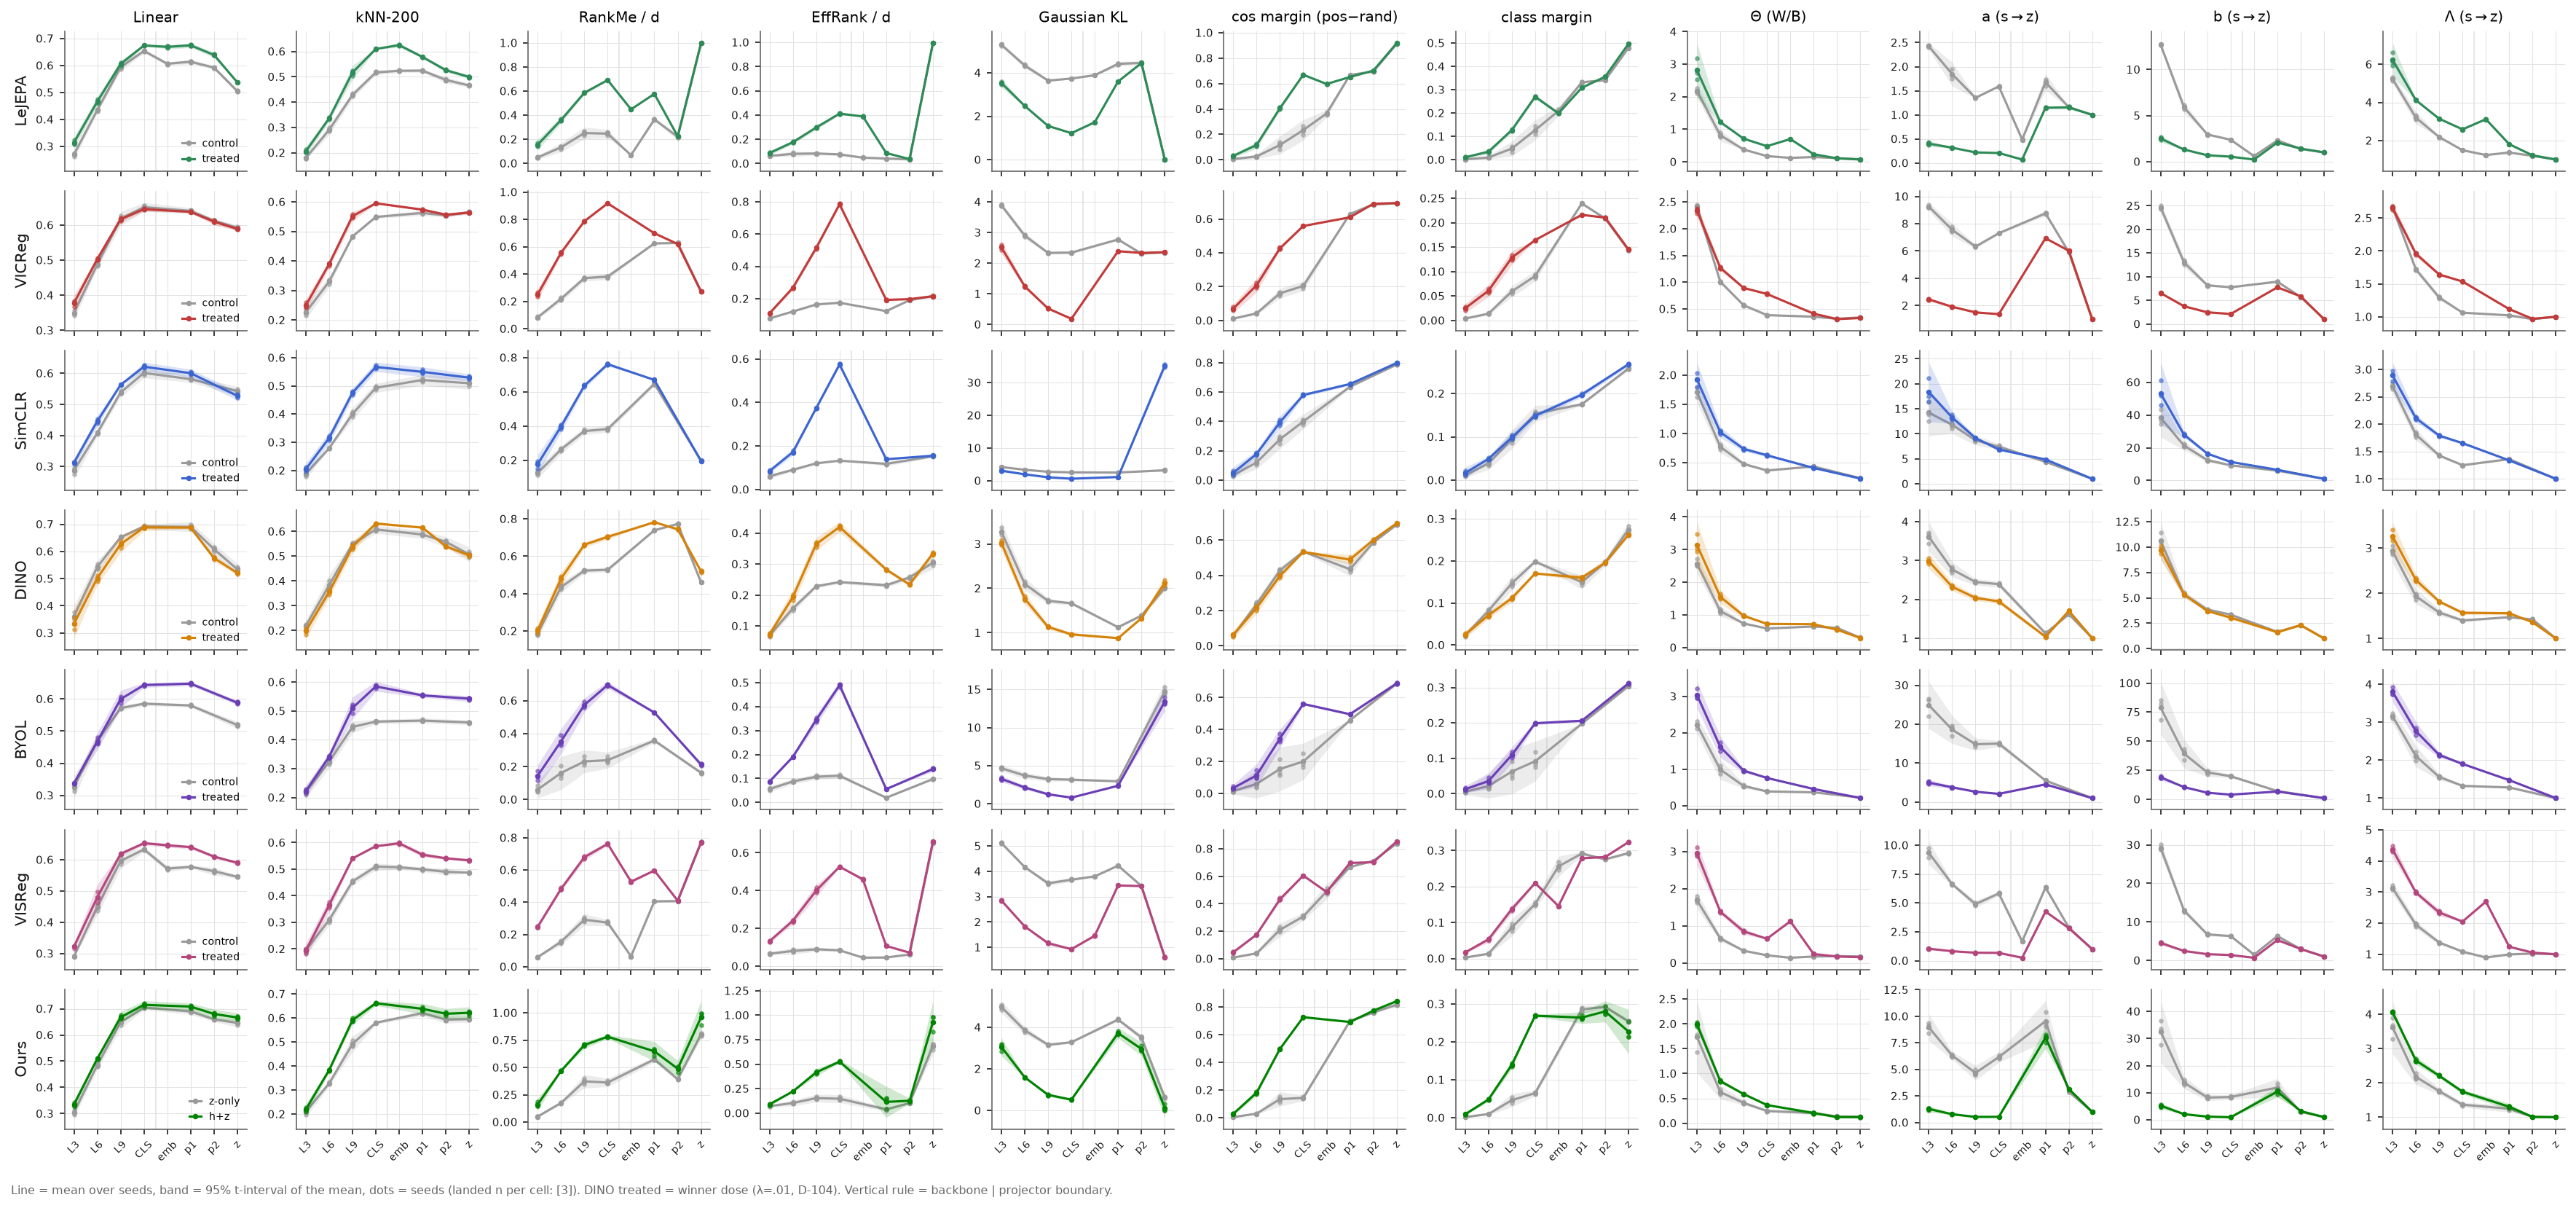
\includegraphics[width=\linewidth]{figures/fig_treatment_appendix.png}
  \caption{Full treatment comparison across methods and reported representation
  metrics. Main-text figures show the quantities most directly used in the
  argument.}
  \label{fig:treatment-appendix}
\end{figure}


\end{document}
